\clearpage
\setcounter{page}{1}

\section{Einführung Matlab \label{sec:einmat}}



\subsection*{Einführung}

{\bf Was ist \matl\ ?}
\begin{itemize}
\item \matl\ (abkürz. für MATrix LABoratory) ist ein Software-Paket für numerische Berechnung und Visualisierung.
Es besteht aus einer großen Anzahl an vorgefertigten Funktionen (z.B. lineare Algebra, Lösen von Differentialgleichungen, ...)

\item  Bei \matl\ steht der Fokus mehr auf numerischer Berechnung, während die Funktionalität von {\sc Maple} und {\sc Mathematica} beispielsweise mehr auf symbolische Algebera ausgerichtet ist.

\item Bekannte \matl-ähnliche Open-Source Programme: {\sc Scilab}, {\sc Octave}
\end{itemize}


{\bf Grund-Features:}
\begin{itemize}
\item Automatische Dimensionierung (d.h., keine Dimensionsangaben bei Deklaration von Vektoren und Arrays erforderlich)

\item Case-Sensitive (d.h., \verb(a( und \verb(A( sind unterschiedliche Variablen)

\item Eingebaute Funktionen basieren auf Vektor- und Matrixoperationen und sind dementsprechend auch für diese optimiert.

\item Datei-Typen:
\begin{itemize}
 \item M-Dateien: Standard ASCII Textdateien mit \verb(.m( -Dateiendung
 \item Mat-Dateien: Binärdateien, mit \verb(.mat( -Dateiendung
 \item Mex-Dateien (``\matl-Executable''): C, C++ oder Fortran Programme, welche von \matl\ aufgerufen werden können
\end{itemize}

\item Grundlegendes Daten-Objekt ist das Array, welches aus Unterelementen verschiedenster Typen (Integern, Doubles, Matrizen, Characters, Strings, Strukturen und Zellen) bestehen kann.

\item Der Typ einzelner Daten-Objekte muss nicht explizit deklariert werden. (z.B. besteht auch keine Notwendigkeit Variablen als Reel oder Komplex zu deklarieren)
\end{itemize}



\clearpage %%%%%%%%%%%%%%%%%%%%%%%%%%%%%%%%%%%%%%%%%%%%%%%%%%%%%%%%%%%%%%%%%%%%%%%%%%%
\subsection*{Grundbefehle}

\begin{tabular}{ll}
\multicolumn{2}{c}{\bf Hilfe}\\ 
\urule{2}
\verb(help <command>( & Hilfe zu \verb(<command>(\\
\verb(lookfor <string>( & listet Hilfe zu \verb(<string>( auf\\
\midrule
\end{tabular}\smallskip

\begin{tabular}{ll}
\multicolumn{2}{c}{\bf Verzeichnisbefehle}\\
\urule{2}
\verb(pwd( & aktuelles Verzeichnis anzeigen\\
\verb(cd( & Verzeichnis ändern\\
\verb(dir( / \verb(ls( & Inhalt des aktuellen Verzeichnisses anzeigen\\
\midrule
\end{tabular}\medskip

\underline{Beispiel:}

{\small\begin{verbatim}
>> help cos
 COS    Cosine.
    COS(X) is the cosine of the elements of X. 
 Overloaded methods
    help sym/cos.m
 \end{verbatim}}

 
 
\subsection*{Variablen}

\begin{tabular}{ll}
\multicolumn{2}{c}{\bf Operatoren}\\
\urule{2}
\verb(=( & einen Wert zuweisen\\
\verb(+ - * / ^( & Rechenoperatoren\\
\verb(,( (am Ende der Zeile) & Befehl mit Output\\
\verb(;( (am Ende der Zeile) & kein Output\\
\verb(...( & Zeilenumbruch innerhalb eines Befehls\\
\midrule
\end{tabular}\smallskip

\begin{tabular}{ll}
\multicolumn{2}{c}{\bf Konstanten}\\
\urule{2}
\verb(i,j( & Imaginärwert $\sqrt{-1}$\\
\verb(pi( & $\pi = 3.14\ldots$\\
\verb(inf(  & Unendlich $\inf$\\
\verb(NaN(  & not a Number, z.\ B.\ $\frac{0}{0}$\\
\verb(eps( & kleinste positive Zahl, welche sich ausgeben lässt\\
\midrule
\end{tabular}\smallskip

\begin{tabular}{ll}
\multicolumn{2}{c}{\bf Variablenmanagement}\\
\urule{2}
\verb(who( & listet die Namen aller im Workspace befindlichen Variablen auf\\
\verb(whos( & listet Namen und Größe der Variablen\\
\verb(clear( & clear Workspace\\
\verb(clear <var>( & clear Variable \verb(<var>(\\
\verb(clc( / \verb(clf( / \verb(cla( & clear command / figure / axes\\
\midrule
\end{tabular}\medskip

Für mehr Informationen: Eingabe von \verb/help +/ in \matl-Kommandozeile.\medskip

\underline{Beispiele:}\medskip

\begin{minipage}[t]{0.5\textwidth}
\small\begin{verbatim}
>> ( 47 + 1e+02 * 1.5 + 4^2 ) / 4
ans =
   53.2500
\end{verbatim}
\end{minipage}
\hfill
\begin{minipage}[t]{0.49\textwidth}
Die Variable \verb(ans( ist das Ergebnis der letzten Rechenoperation.
\end{minipage}\medskip

\begin{minipage}[t]{0.5\textwidth}
{\small\begin{verbatim}
>> a = ( 47 + 1e+02 * 1.5 + 4^2 ) / 4
a =
   53.2500
\end{verbatim}}
\end{minipage}
\hfill
\begin{minipage}[t]{0.49\textwidth}
Das Ergebnis wird in Variable \verb(a( gespeichert.
\end{minipage}

 
 
\subsection*{Mathematische Funktionen}

\begin{tabular}{ll}
\urule{2}
\verb/sqrt(x)/ & Quadratwurzel\\
\verb/xp(x)/ & Exponentialfunktion\\
\verb/log(x)/ / \verb/log10/ & Logarithmusfunktionen\\
\verb/sin(x)/ & Sinus\\
\verb/cos(x)/ & Cosinus\\
\verb/tan(x)/ & Tangens\\
\verb/atan(x)/ & Arkustangens (Winkel $-90^{\circ}\ldots+90^{\circ}$)\\
\verb/atan2(y,x)/ & Arkustangens (Winkel $-180^{\circ}\ldots+180^{\circ}$)\\
\verb/abs(x)/ & Betrag von \verb/x/\\
\verb/sign(x)/ & Signum (Vorzeichen von \verb/x/)\\
\midrule
\end{tabular}\medskip

Mehr Infos: Eingabe von \verb/help elfun/ oder
\verb/help datafun/ in \matl-Kommandozeile.\medskip


\underline{Beispiel:}\medskip

\begin{verbatim}
>> y1 = 2^2+log(pi)*sin(0.75*pi/2)+sqrt(exp(2*pi/3))
\end{verbatim}

\begin{minipage}[b]{0.5\textwidth}
\begin{verbatim}
y1 =
    7.9072
\end{verbatim}
\end{minipage}
\hfill
\begin{minipage}[b]{0.46\textwidth}
$$ y_1 = 2^2 + \ln \pi \sin(0.75\pi/2) + \sqrt{e^{2/3\pi}}$$
\end{minipage}
 
 
 
\clearpage %%%%%%%%%%%%%%%%%%%%%%%%%%%%%%%%%%%%%%%%%%%%%%%%%%%%%%%%%%%%%%%%%%%5
\subsection*{Vektoren und Matrizen}

\begin{tabular}{ll}
\multicolumn{2}{c}{\bf Vektor- und Matrixbefehle}\\
\urule{2}
\verb/[ x1 x2 ...; y1,y2,...] / & Vektor oder Matrix ('\verb/,/' oder Leerzeichen zwischen\\
 &  Spalten, '\verb/;/' oder Zeilenumbruch zwischen Reihen)\\
\verb/start: <stepsize:> end/ & Spaltenoperator (\verb/stepsize/ opt., sonst = 1)\\
\verb/linspace(start,end,num_steps)/ & linearer Zeilenvektor\\
\verb/logspace(start,end,num_steps)/ & logarithmischer Zeilenvektor\\
\verb/eye(rows,columns)/ & Einheitsmatrix [Zeilen x Spalten]\\
\verb/ones(rows,columns)/ & Matrix, bei der alle Einträge=1 sind [Zeilen x Spalten]\\
\verb/zeros(rows,columns)/ & Nullmatrix [Zeilen x Spalten]\\
\verb/rand(rows,columns)/ & Matrix mit Zufallswerten [Zeilen x Spalten]\\
\verb/a(index)/ & Element des Vektors \verb/a/ an Position \verb/index/\\
\verb/A(r,c)/ & Element der Matrix \verb/A/ an Position \verb/r/ x \verb/c/\\
\midrule
\end{tabular}\medskip

\underline{Beispiele:}\medskip

\begin{minipage}[t]{0.5\textwidth}
\small\begin{verbatim}
>> x=[1 2 3]
x =
     1     2     3
>> y=[4;5;6]
y =
     4
     5
     6
>> A=[1 2 3;4,5,6;7 8,9]
A =
     1     2     3
     4     5     6
     7     8     9
>> A(2,3)
ans =
     6
\end{verbatim}
\end{minipage}
 \hfill
\begin{minipage}[t]{0.42\textwidth}
\small\begin{verbatim}
>> A(1,2)=8
A =
     1     8     3
     4     5     6
     7     8     9
>> B=A(2:3,1:3)
B =
     4     5     6
     7     8     9
>> v=0:2:8
v =
     0     2     4     6     8
>> v=[8:-2:0]
v =
     8     6     4     2     0
\end{verbatim}
\end{minipage}


% \subsection*{Vektor- und Matrixoperationen}

\begin{tabular}{ll}
\multicolumn{2}{c}{\bf Operationen}\\
\urule{2}
\verb(.* .\ ./ .^( & elementweise Berechnung\\
\verb(\ /( & linke und rechte Division\\
\verb/transpose(A)/ oder \verb/A.'/ & Transponierte von \verb/A/\\
\verb/ctranspose(A)/ or \verb/A'/ & Transponierte von \verb/A/ (komplex Konjugiert)\\
\verb/inv(A)/ & Inverse von \verb/A/\\
\verb/det(A)/ & Determinante von \verb/A/\\
\midrule
\end{tabular}\smallskip

\begin{tabular}{ll}
\multicolumn{2}{c}{\bf Dimensionen}\\
\urule{2}
\verb/[M,N] = SIZE(A)/ & Dimension von Matrix und Vektor\\
\verb/M = SIZE(A,DIM)/ & Länge der Komponente \verb/DIM/ der Matrix \verb/A/ \\
\midrule
\end{tabular}\smallskip

\begin{tabular}{ll}
\multicolumn{2}{c}{\bf Mathematische Funktionen von Vektoren und Matrizen}\\
\urule{2}
\verb/sum(a)/ & Summe der Vektorelemente\\
\verb/prod(a)/ & Produkt der Vektorelemente\\
\verb/min(a)/ & kleinstes Vektorelement\\
\verb/max(a)/ & größtes Vektorelement\\
\verb/sort(a)/ & Elemente in aufsteigender Reihenfolge\\
\verb/find(a)/ & nicht-Null Elemente\\
\midrule
\end{tabular}\medskip

\underline{Beispiele:}\medskip

\begin{minipage}[t]{0.5\textwidth}
\small\begin{verbatim}
>> A=[1 2 3; 4 5 6; 7 8 9];
>> B=[1 2 3; 2 4 5; 3 7 8];
>> b=[2 4 6 8 10]';
>> v=0:2:8;

>> v*b
ans =
   160
>> v'*b'
ans =
     0     0     0     0     0
     4     8    12    16    20
     8    16    24    32    40
    12    24    36    48    60
    16    32    48    64    80
\end{verbatim}
\end{minipage}
\hfill
\begin{minipage}[t]{0.42\textwidth}
\small\begin{verbatim}
>> c=v+b';
>> c=v-b';
>> C=A+B;
>> C=A-B;
>> C=A*B;
>> c=A*v(1:3)'
c =
    16
    34
    52
>> c=v.*b'
c =
     0     8    24    48    80
\end{verbatim}
\end{minipage}\bigskip

\underline{Beispiel:}\medskip

\begin{minipage}[t]{0.4\textwidth}
\small\begin{verbatim}
>> A=[5 -3 2; -3 8 4; 2 4 -9];
>> b=[10;20;9];
>> x=A\b
x =
    3.4442
    3.1982
    1.1868
\end{verbatim}
\end{minipage}
\hfill
\begin{minipage}[t]{0.59\textwidth}
Lösen des linearen Gleichungssystems: $\bA\bx = \bb$
\begin{eqnarray*}
5x &=& 3y-2z+10\\
8y+4z &=& 3x+20\\
2x+4y-9z &=& 9\\
\end{eqnarray*}
\end{minipage}



\clearpage
\subsection*{Skripte und Funktionen}

\begin{itemize}
\item Skript:\\
  Wenn ein Skript aufgerufen wird, führt \matl\ schlicht die in der Datei befindlichen Befehle aus.
  Skripte können im Workspace bereits vorhandene Daten bearbeiten oder auch neue Daten erzeugen.
  Auch wenn Skriptdateien keine Outputargumente aufweisen, werden alle erzeugten Variablen im Workspace gespeichert und können in darauffolgenden Rechenoperationen verwendet werden.
\item Funktion:\\
  Funktionen sind \verb/.m/-Dateien, welche Inputargumente aufnehmen und Outputargumente wiedergeben.
  Der Name der \verb/.m/-Datei und der Funktion sollten übereinstimmen.
  Funktionen arbeiten mit lokalen Variablen in einem funktioneigenen Worskpace unabhängig des von der \matl-Kommandozeile bearbeiteten Workspaces.
\end{itemize}
Sowohl Skripte als auch Funktionen werden als .m-Datei gespeichert.\medskip

\underline{Struktur von Funktionen:}
{\small\begin{verbatim}
function [a_out,b_out] = name_of_function(a_in,b_in)
%         output list                     input list
%
% Description of function can be placed here
% by using the comment-operator '%'. This
% informations can be displyed by typing
% 'help name_of_function' at MATLAB-command-line.
.
.
a_out = a_in - a_out;
b_out = a_in + a_out;
.
.
\end{verbatim}}

\underline{Beispiel: Länge eines Vektors berechnen}
{\small\begin{verbatim}
function vlength = fvectorlength(vector)
%
% Computation of the length 'vlength' of
% a column vector 'vector'

vlength = sqrt(vector'*vector);
\end{verbatim}}
Aufrufen der Funktion:
{\small\begin{verbatim}
>> fvectorlength([-1;3;5])
ans =
    5.9161
\end{verbatim}}



\clearpage %%%%%%%%%%%%%%%%%%%%%%%%%%%%%%%%%%%%%%%%%%%%%%%%%%%%%%%%%%%%%%%%%%%%%%%%%%%%%%%%%%%%%%5
\subsection*{Logikoperatoren}

\begin{tabular}{llll}
\urule{4}
\verb(== , ~=( & gleich, nicht gleich\\
\verb(< , <=( & kleiner als, kleiner gleich\\
\verb(> , >=( & größer als, größer gleich\\
\midrule
\verb/~/ & logisches NOT & \verb/&/ & elementweise logiesches AND\\
\verb/|/ & elementweise logisches OR & \verb/xor/ & logisches EXCLUSIVE-OR\\
\midrule
\end{tabular}\medskip

Mehr Infos: Eingabe von \verb/help +/ in \matl-Kommandozeile.




\subsection*{IF-/Fallunterscheidungen und Schleifen}

\begin{tabular}{ll}
\urule{2}
\verb(IF( expression (z.B. \verb/a==1/)& IF-Statement Bedingung\\
  \hspace*{0.3cm} statements\\
\verb(ELSEIF( expression & ELSE und ELSEIF sind optional\\
  \hspace*{0.3cm} statements &  \\
\verb(ELSE(\\
  \hspace*{0.3cm} statements\\
\verb(END(\\
\midrule
\verb(SWITCH( switch-expr (z.B. \verb/id/)& SWITCH-Statement Fall \\
\verb(  CASE( case-expr, (z.B. \verb/1/) \\
  \hspace*{0.6cm} statement, ..., statement\\
\verb(  CASE {(case-expr1, case-expr2, case-expr3,...\verb(}(\\
  \hspace*{0.6cm} statement, ..., statement\\
\verb(  OTHERWISE,(\\
  \hspace*{0.6cm} statement, ..., statement\\
\verb(END(\\
\midrule
\verb(FOR( variable = expr (z.B. \verb/ii=1:10/)& Wiederholung der Statements\\
  \hspace*{0.3cm} statement, ..., statement & in einer spezifischen Anzahl.\\
\verb(END(\\
\midrule
\verb(WHILE( expression (z.B. \verb/ii<imax/)& Wiederholung der Statements eine  \\
  \hspace*{0.3cm} statements & unbestimmte Anzahl bis Bedingnung erfüllt.\\
\verb(END(\\
\midrule
\end{tabular}



\clearpage %%%%%%%%%%%%%%%%%%%%%%%%%%%%%%%%%%%%%%%%%%%%%%%%%%%%%%%%%%%%%%%%%%%%%%%%%%%%%
\subsection*{Plotten von Schaubildern}

\begin{tabular}{ll}
\multicolumn{2}{c}{\bf Bedienen des 'figure'-Fensters}\\
\urule{2}
\verb/figure , figure(no)/ & erstellen, aktivieren eines Schaubilds mit Nummer \verb/no/\\
\verb/subplot(num_rows,num_cols,index)/ & erstellen eines Subplots\\
& z.B., \verb/subplot(2,3,2)/: Subplot mit 2 Zeilen\\
& und 3 Spalten, aktivieren eines 2. Subplots\\
\verb/gcf/ & 'get current figure'\\
\verb/clf/ & 'clear active figure'\\
\verb/delete(id)/ & Objekte mit \verb(id( löschen\\
\verb/close(index)/ & 'figure'-Fenster Nr. \verb(index( löschen\\
\verb/close all /& alle 'figure'-Fenster löschen\\
\verb/hold <on | off>/ & aktuelles 'figure'-Fenster geöffnet lassen\\
& bei Generierung neuer Plots an/aus \\
\midrule
\end{tabular}\smallskip

\begin{tabular}{ll}
\multicolumn{2}{c}{\bf 2-D Plot Befehle}\\
\urule{2}
\verb/plot(<x,>y<,plotstyle>/,...) & Plot, Linear (\verb/<>/ = opt.)\\
\verb/fplot(func,range)/ & Plot einer expliziten Funktion\\
\verb/line(x,y)/ & erstellen der Linie durch Koordinatenvektoren \verb/x,y/\\
\verb/text(x,y,string)/ & platzieren von \verb/string/ an Position \verb/x,y/\\ 
\multicolumn{2}{l}{Für mehr Infos über 2-D Plots: aufrufen von {\ttfamily help plot} in Kommandozeile.}\\
\midrule
\end{tabular}\smallskip

\begin{tabular}{ll}
\multicolumn{2}{c}{\bf 3-D Plot Befehle}\\
\urule{2}
\verb/plot3(x,y,z <,plotstyle> ,...)/ & dreidimensionaler Plot\\
\verb/sphere/ & plotten einer Kugel\\
\verb/[x,y,z] = sphere/ & Koordinaten einer Einheitskugel unter \verb/x,y,z/ speichern\\
\verb/line(x,y,z)/ & erstellen einer Linie durch Koordinatenvektoren \verb/x,y,z/\\
\verb/text(x,y,z,string)/ & platzieren von \verb/string/ an Position \verb/x,y,z/\\
\midrule
\end{tabular}\smallskip

\begin{tabular}{lll|lll}
\multicolumn{6}{c}{\bf Plotstyles}\\
\urule{6}
\multicolumn{3}{c}{Farben:} & \multicolumn{3}{c}{Linienstyles:}\\
\verb/k/ schwarz & \verb/r/ rot & \verb/g/ grün & 
\verb/-/ durchgängig    & \verb\o\ Kreis & \verb/./ Punkte\\
\verb/b/ blau  & \verb/m/ magenta & \verb/w/ weiß &
\verb/--/ gestrichelt  & \verb\*\ sterne & \verb\x\ x\\
\verb/c/ cyan  & \verb/y/ gelb & &
\verb/:/ gepunktet   & \verb\+\ plut & \verb/-./ Punkt-Strichlinie\\
Mehr Infos: \verb/help plot/\\
\midrule
\end{tabular}\bigskip

\begin{minipage}[c]{0.54\textwidth}
\underline{Beispiele:}
\small\begin{verbatim}
>> figure(1)
>> clf
>> t=0:pi/20:2*pi;
>> plot(t,sin(t),'-.r*')
>> hold on
>> plot(t,(sin(t-pi/2)),'linestyle','--',...
   'marker','o','color','m')
>> plot(t,sin(t-pi),':bs')
>> hold off
\end{verbatim}
\end{minipage}
\hfill
\begin{minipage}[c]{0.45\textwidth}
\centering
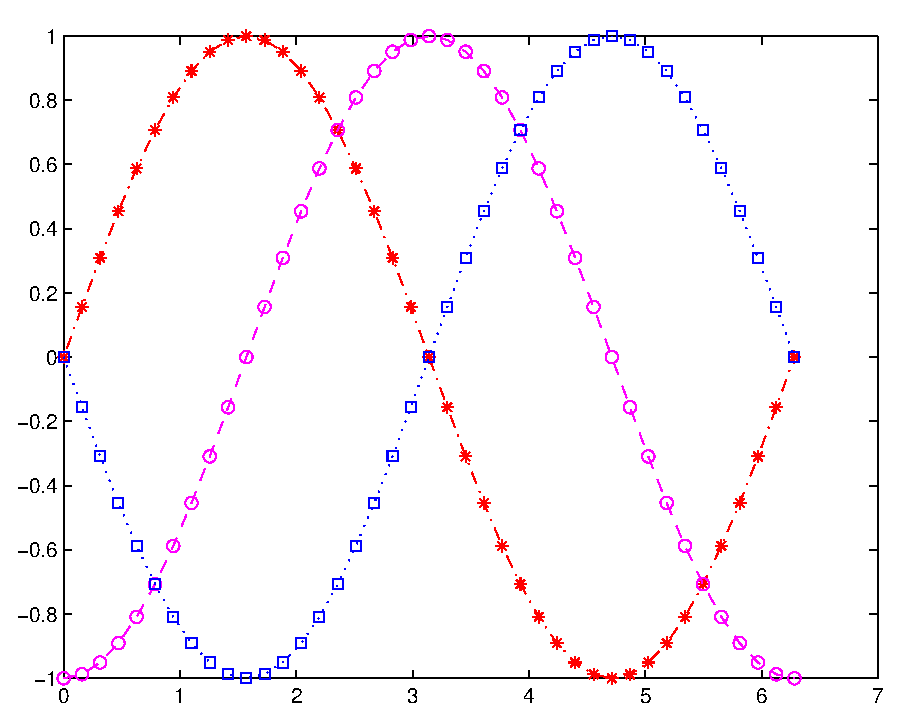
\includegraphics[width=0.8\textwidth]{fig/ue3_plot_example.eps}
\end{minipage}\bigskip

\begin{tabular}{ll}
\multicolumn{2}{c}{\bf Labeln von Achsen und Figures}\\
\urule{2}
\verb/axis([xmin,xmax,ymin,ymax<,zmin,zmax>)/ & Skalierung (min=\verb/-inf/ oder\\
& max=\verb/inf/ $\rightarrow$ Auto Skalierung) \\
\verb/axis <on | off | auto | equal | square>/ & verschiedene Achsen-Befehle\\
& Mehr: \verb/help axis/\\
\verb/grid <on | off>/ & Gitter an/aus\\
\verb/gca/ & Wiedergabe der aktuellen Achse\\
\verb/cla/ & löschen der aktuellen Achse\\
\verb/xlabel(string)/ & Label der x-Achse\\
\verb/ylabel(string)/ & Label der y-Achse\\
\verb/zlabel(string)/ & Label der z-Achse\\
\verb/title(string)/ & Titel der aktuellen Achse\\
\verb/legend(string_1,string_2,...<,pos>)/ & Legende platzieren\\
& \verb/pos = 0,1,2,3,4,-1/\\
\midrule
\end{tabular}



\clearpage %%%%%%%%%%%%%%%%%%%%%%%%%%%%%%%%%%%%%%%%%%%%%%%%%%%%%%%%%%%%%%%%%%%%%%%%%%%%%%%%%%%%%%%%%%%%%
\subsection{Animation eines rotierenden Kragarms}

\begin{minipage}[t]{0.5\textwidth}
Ein Kragarm der Länge $L$ ist am oberen Ende (Punkt P2) an einer vertikalen Stange (höhe H) befestigt.
Der Kragarm ist im Winkel $\alpha$ zur Stange geneigt.
Die Stange ist am unteren Ende (Punkt P1) drehbar gelagert mit der $z$-Achse als Rotationsachse.
Am Freien Ende des Kragarms (Punkt P3) ist eine Kugel mit dem Radius $R$ befestigt.\smallskip

Programmieren Sie ein \matl-Skript (\verb/.m/-file), in welchem die Rotation $\varphi$ um die $z$-Achse des dargestellten Systems in animierter Form dargestellt wird.
\end{minipage}
\hfill
\begin{minipage}[t]{0.39\textwidth}
\begin{picture}(0,0)
\unitlength1cm
% \includegraphics{fig/bild1020.pdf}
 \put(0.0,-5.0){\scalebox{0.8}{\input{fig/ue3_bild1020.pdf_t}}}
\end{picture}
\end{minipage}\bigskip

\textit{Hinweis:} Nutzen sie die Rotationsmatrix 

\ebn
 \bR =
 \begin{bmatrix}
       \cos{\varphi} & -\sin{\varphi} &     0 \\
       \sin{\varphi} & \cos{\varphi}  &     0 \\
        0            &      0         &     1
 \end{bmatrix},
\een

welche mit $\bar{\bv}=\bR \smpc \bv$ die Rotation eines Vektors $\bv$ um die $z$-Achse beschreibt.

\subsection{Animation mithilfe einer Subroutine}

Das \matl-Skript aus der vorherigen Aufgabe soll nun modifiziert werden.
Eine selbst programmierte Funktion soll die rotierten Koordinaten für die Animation berechnen.
Input parameter sollen die die Ursprungskoordinaten und der Rotationswinkel $\varphi$ sein.
Der Output der Funktion sollten die Koordinaten des rotierten Systems sein.
